% !TeX spellcheck = en_US

\section{Stability Analysis}

A first indicator of the stability of a walking system is the maximum displacement on the ordinate axis, as bigger oscillations tend to be related with poor robustness of the stability of the gait. Figure~\ref{fig:displacement} shows the trajectory of the~\glsxtrshort{com}, with the help of which a first impression of the stability can be gained, as the~\glsxtrshort{com} remains between $\gls{y}_{min}$ and $\gls{y}_{max}$ at every instant. Note that the vertical displacement remains relatively continuous at the upper end, while strong oscillations occur at the lower end. In figure~\ref{fig:displacement-zoom} a section of the vertical displacement is shown, where it can be seen that the robot reaches a negative horizontal displacement at the lower end, causing a loop. This is far from an ideal gait and is extremely energy consuming. \\

A quantitative analysis of the stability of the system can be achieved by evaluating the phase diagram\footnote{A phase diagram typically consists of a set of curves or trajectories that represent the time evolution of the system's state. Each trajectory represents the path that the system would follow in the phase space for a particular set of initial conditions. By plotting multiple trajectories with different initial conditions, it is possible to visualize the range of possible behaviors of the system.~\cite{Goswami1996}}. In a phase plot, each point in the phase space represents a unique state of the system, defined by the values of its state variables. If during each step the trajectory of the system in the phase plot tends to the limit cycle\footnote{The limit cycle is a type of behavior exhibited by some dynamical systems, in which the system oscillates or repeats its behavior indefinitely, but without necessarily converging to a steady state or equilibrium~\cite{Goswami1996}.}, the system is stable,~\ie the system will converge to the limit cycle regardless of the initial conditions, and the limit cycle will persist indefinitely. In an unstable limit cycle, on the other hand, the trajectory will approach the limit cycle for some initial conditions, but it will diverge from it for others. The existence of a limit cycle in the phase plot thus ensures (marginal) stability.~\cite{Goswami1996} Figure~\ref{fig:phase-plot} shows the phase plot of the simulation,~\ie the graphical representation of the behavior of the dynamical system in the phase space\footnote{The phase space refers to the set of all possible states of a system.}. The plot shows the position of the torso of the JenaFox robot on the sagittal plane (\ie the plane spanned between the abscissa axis (X-axis, orange) and ordinate axis (Y-axis, green), see figure~\ref{fig:coordinate-system}) during its motion and reveals that the robot is asymptotically stable in its gait. The simulation was stopped as soon as the robot reached a distance of $15\,\textrm{\si{\metre}}$. The vertical displacement of the torso in$~\left[\si{\metre}\right]$ is plotted on the abscissa axis, the vertical velocity in$~\left[\si{\metre\per\second}\right]$ on the ordinate axis, respectively.

\begin{figure}[H]%
    \centering%
    \begin{subfigure}[t]{0.74\linewidth}%
        \centering%
        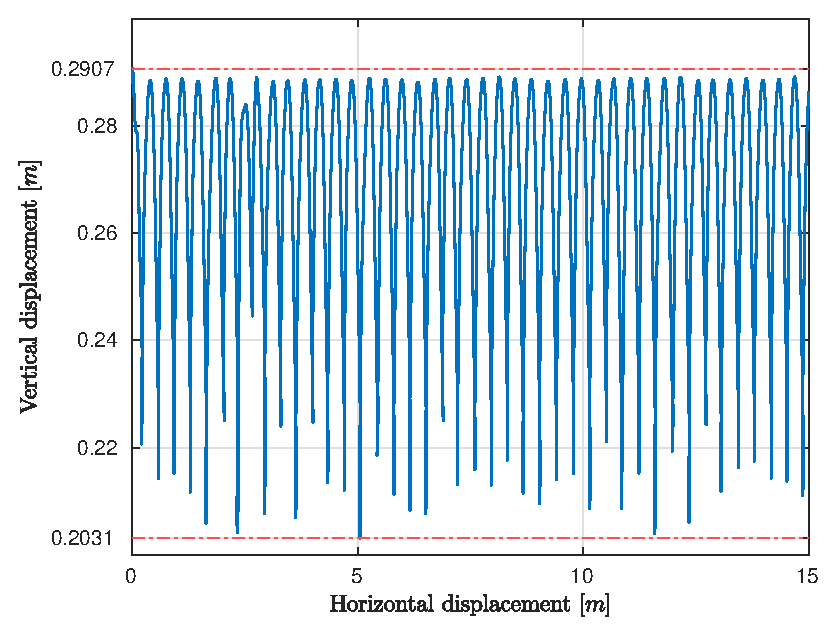
\includegraphics[width=\linewidth]{displacement/displacement.eps}
        \caption{The full trajectory of the~\glsxtrshort{com} over the course of $15\,\textrm{\si{\metre}}$. Note that the vertical displacement remains relatively continuous at the upper end, while strong oscillations occur at the lower end.}%
        \label{fig:displacement-full}%
        \vspace*{2mm}%
    \end{subfigure}%
    %
    \vfil%
    %
    \begin{subfigure}[b]{0.74\linewidth}%
        \centering%
        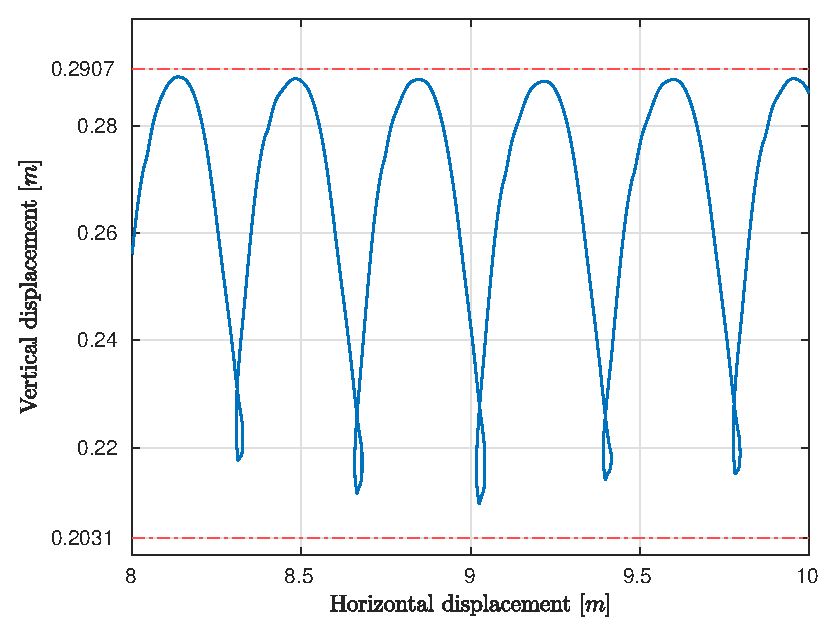
\includegraphics[width=\linewidth]{displacement/displacement-zoom.eps}
        \caption{A section of the~\glsxtrshort{com} trajectory is shown, where it can be seen that the robot reaches a negative horizontal displacement at the lower end, causing a loop. This is far from an ideal gait and is extremely energy consuming.}%
        \label{fig:displacement-zoom}%                      
    \end{subfigure}%
    %
    \caption{The trajectory of the~\glsxtrfull{com}, with the help of which a first impression of the stability can be gained, as bigger oscillations tend to be related with poor robustness of the stability of the gait. The simulation was stopped after a distance of $15\,\textrm{\si{\metre}}$ was reached (\subref{fig:displacement-full}). A more detailed section of the trajectory reveals a negative horizontal displacement at the lower end (\subref{fig:displacement-zoom}). The horizontal displacement of the torso in$~\left[\si{\metre}\right]$ is plotted on the abscissa axis, the vertical displacement in$~\left[\si{\metre}\right]$ on the ordinate axis, respectively.}%
    \label{fig:displacement}%
\end{figure}%
% \noindent

\begin{figure}[H]%
    \centering%
    \begin{subfigure}[t]{0.8\linewidth}%
        \centering%
        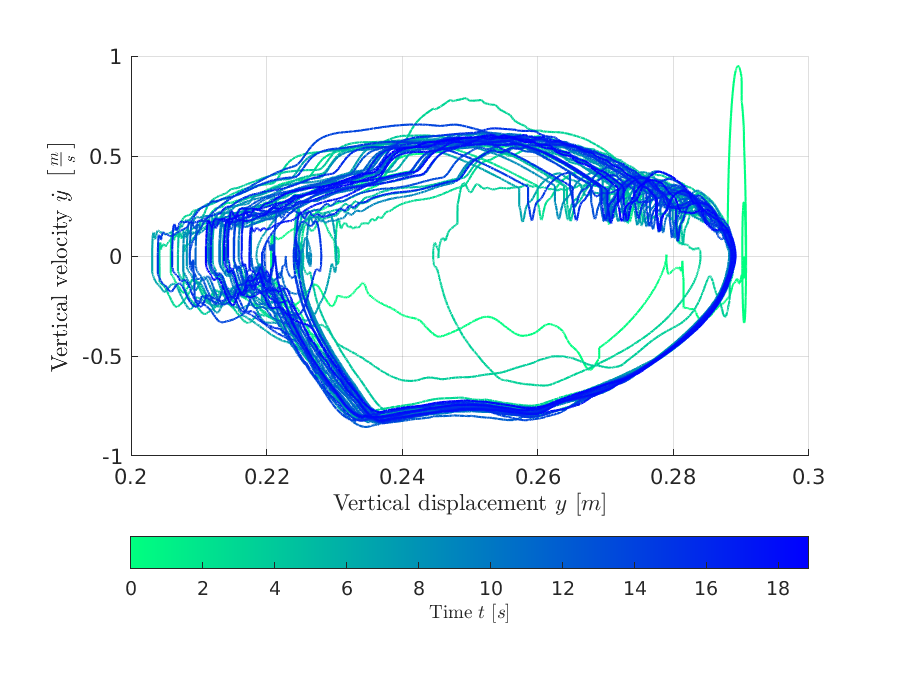
\includegraphics[width=\linewidth]{phase-plot/phase-plot.eps}
        \caption{The phase plot of the simulation. The simulation was stopped after a distance of $15\,\textrm{\si{\metre}}$ was reached. Time is represented by a colormap, which shows that the robot converges to an asymptotically stable gait with few oscillations.}%
        \label{fig:phase-plot-time}%
        \vspace*{2mm}%
    \end{subfigure}%
    %
    \vfil%
    %
    \begin{subfigure}[b]{0.8\linewidth}%
        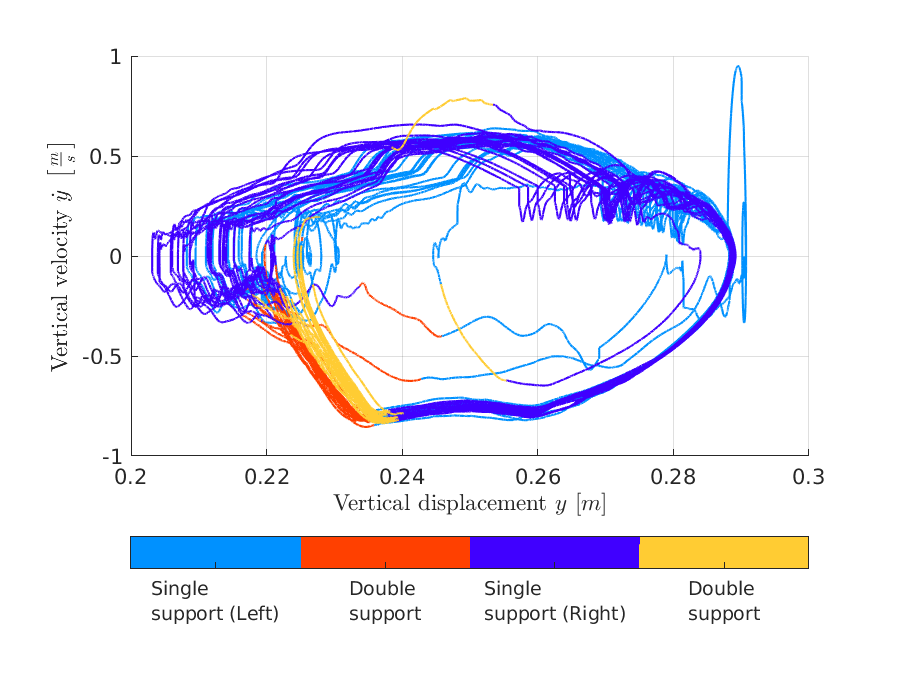
\includegraphics[width=\linewidth]{phase-plot/phase-plot-ground-state.eps}
        \caption{The phase plot of the simulation. The simulation was stopped after a distance of $15\,\textrm{\si{\metre}}$ was reached. The ground state of the system is represented by a colormap, showing the two single support phases (light blue, dark blue) and the two double support phases (red, yellow).}%
        \label{fig:phase-plot-ground-state}%
    \end{subfigure}%
    %
    \caption{The phase plot of the simulation,~\ie the graphical representation of the behavior of the dynamical system in the phase space over the entire simulation with color-encoded time (\subref{fig:phase-plot-time}) and ground state (\subref{fig:phase-plot-ground-state}). The plot shows the position of the torso of the JenaFox robot on the sagittal plane during its motion and reveals that the robot is asymptotically stable in its gait. The vertical displacement of the torso in$~\left[\si{\metre}\right]$ is plotted on the abscissa axis, the vertical velocity in$~\left[\si{\metre\per\second}\right]$ on the ordinate axis, respectively.}%
    \label{fig:phase-plot}%
\end{figure}%
% \noindent
